% ============================================================
%  Diapositivas de respaldo (barras rojas)
%  Se muestran al final; cada una recupera su numero original.
% ============================================================

\setcounter{framenumber}{7}
\makered
\begin{frame}{Etapa 1: Bolivia -- evolución de la predicción}
  \begin{center}
    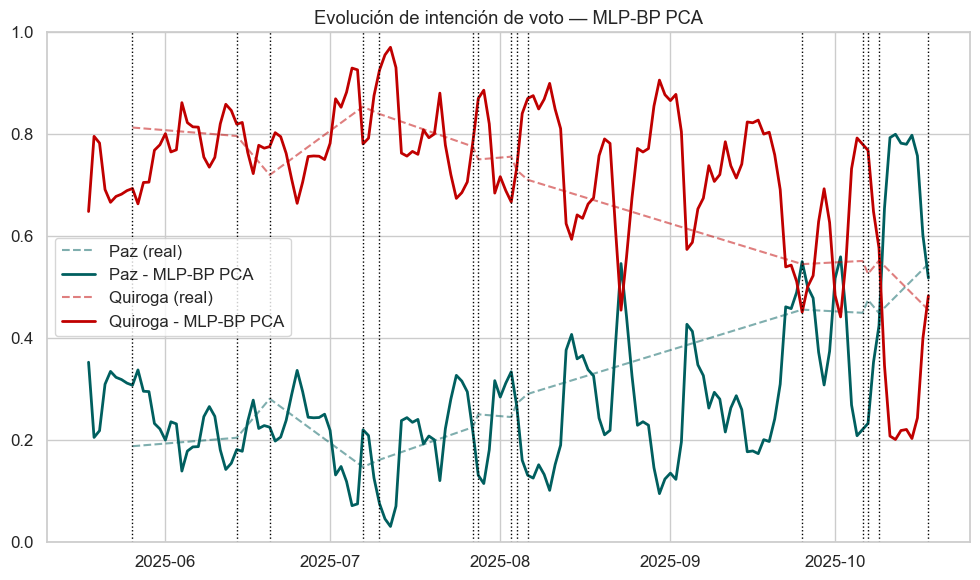
\includegraphics[width=0.88\textwidth]{img/mlp_bp_pca_timeseries.png}
  \end{center}
  {\footnotesize\color{subtleGray}\centering
    Evolución predicha vs.\ encuestas -- MLP-BP+PCA (modelo ganador)}
\end{frame}
\makeblue

\setcounter{framenumber}{12}
\makered
\begin{frame}{Etapa 2: Parámetros Weibull calibrados por plataforma}
  \begin{columns}[T]
    \begin{column}{0.46\textwidth}
      \begin{center}
      {\setlength{\tabcolsep}{3pt}
      \small
      \rowcolors{2}{tableBand}{white}
      \begin{tabular}{L{2.0cm} C{1.0cm} C{1.0cm} C{1.3cm} C{0.9cm}}
        \toprule
        \rowcolor{barBlue}
        {\color{white}\textbf{Plataforma}} &
        {\color{white}$k$} &
        {\color{white}$\alpha$} &
        {\color{white}$t_0$ (h)} &
        {\color{white}$R^2$} \\
        \midrule
        Facebook   & 0,948 & 0,823 & 46 & 0,351 \\
        Instagram  & 1,137 & 0,521 &  1 & 0,403 \\
        TikTok     & 1,327 & 0,512 & 19 & 0,351 \\
        Twitter/X  & 1,445 & \alrt{1,142} & 6 & 0,691 \\
        \bottomrule
      \end{tabular}}
      \end{center}
      \vspace{0.2em}
      {\footnotesize\color{subtleGray}
        Twitter/X: $\alpha > 1$, tasa creciente (retweet acumulativo)}
    \end{column}
    \begin{column}{0.50\textwidth}
      \textbf{Hallazgo clave para la validez del diseño:}
      \begin{itemize}
        \item La curva de la candidata \textbf{ganadora} (Laura Fernández) es morfológicamente \textbf{idéntica} a la del resto
        \item Sin diferencia estadísticamente significativa entre ganadores y perdedores en ningún día del panel
        \item El patrón de crecimiento es propiedad de la \textbf{plataforma}, no del candidato ni del resultado
      \end{itemize}
      \vspace{0.3em}
      \begin{exampleblock}{\textbf{P2}: Respondida}
        Los parámetros calibrados en Costa Rica 2026 son transferibles
        para reconstruir el histórico de interacciones de \textit{cualquier}
        elección colombiana pasada.
      \end{exampleblock}
    \end{column}
  \end{columns}
\end{frame}
\makeblue

\setcounter{framenumber}{14}
\makered
\begin{frame}{Etapa 2: Precisión del restaurador temporal}
  \textbf{MAPE mediano por plataforma y día de observación}
  \vspace{0.3em}
  \begin{center}
  {\setlength{\tabcolsep}{4pt}
  \scriptsize
  \rowcolors{2}{tableBand}{white}
  \begin{tabular}{L{2.0cm} C{1.5cm} C{1.5cm} C{1.5cm} C{1.7cm} C{1.5cm}}
    \toprule
    \rowcolor{barBlue}
    {\color{white}\textbf{Plataforma}} &
    {\color{white}\textbf{Día 0}} &
    {\color{white}\textbf{Día 1}} &
    {\color{white}\textbf{Día 2}} &
    {\color{white}\textbf{Día 3}} &
    {\color{white}\textbf{Día 7}} \\
    \midrule
    Facebook   & 11,27\% & 6,92\% & 3,73\% & \ok{2,12\%}  & 0,32\% \\
    Instagram  & 64,77\% & \num{20,72\%}$^*$ & 15,67\% & \ok{12,06\%} & 3,76\% \\
    TikTok     & 25,36\% & 14,20\% & 8,35\% & \ok{5,94\%}  & 2,29\% \\
    Twitter/X  & 56,37\% & 11,09\% & 2,55\% & \ok{0,38\%}  & 0,00\% \\
    \bottomrule
  \end{tabular}}
  \end{center}

  \vspace{0.2em}
  {\footnotesize $^*$ Instagram Día 1 = 20,72\%: único que supera el 20\%.
  A partir del \textbf{Día 3}, las cuatro plataformas están por debajo del 13\%. \corr{[Corr.\ 1.10]}}

  \vspace{0.3em}
  \begin{columns}[T]
    \begin{column}{0.52\textwidth}
      \textbf{Criterio adoptado:} día 3 de observación por publicación.\\[0.2em]
      Instagram en Día 3: \ok{12,06\%}; la excepción fue Día 1, no Día 3.
    \end{column}
    \begin{column}{0.44\textwidth}
      \begin{exampleblock}{\textbf{PM3}: Respondida}
        \small La reconstrucción es suficientemente precisa.
        Los parámetros Weibull son transferibles para
        construir datasets de entrenamiento retroactivos.
      \end{exampleblock}
    \end{column}
  \end{columns}
\end{frame}
\makeblue

\setcounter{framenumber}{15}
\makered
\begin{frame}{Etapa 2: Convergencia del error por día de observación}
  \begin{center}
    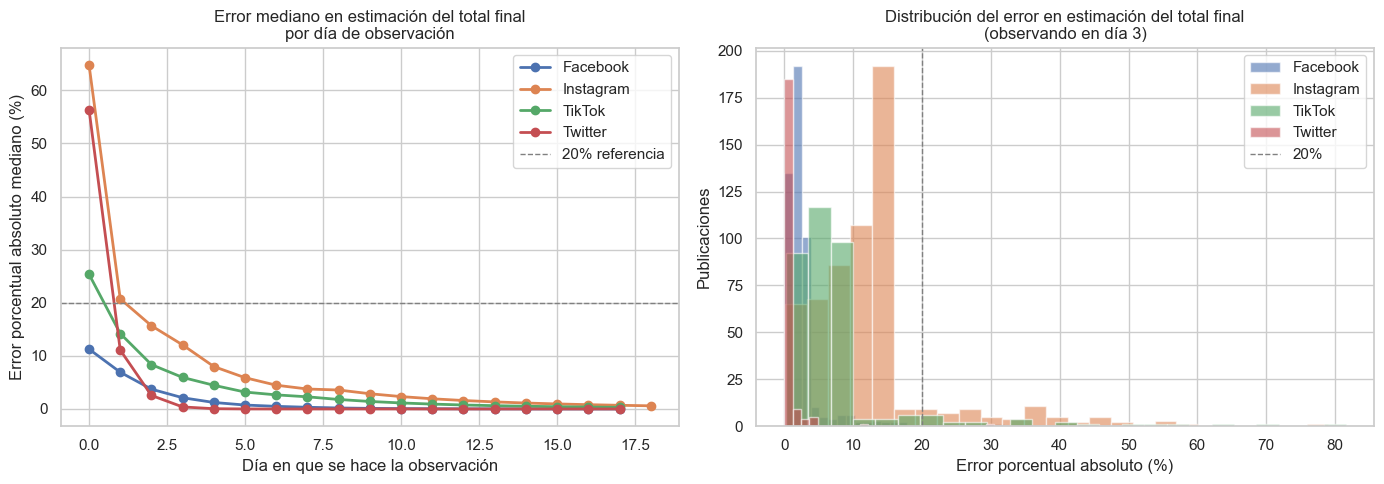
\includegraphics[width=0.88\textwidth]{img/costa_rica_r2_2.png}
  \end{center}
  {\footnotesize\color{subtleGray}\centering
    Izquierda: MAPE mediano por plataforma y día de observación.
    Derecha: distribución de errores individuales en Día 3.
    El 85\% de las publicaciones tiene MAPE $<$ 20\% en Día 3.}
\end{frame}
\makeblue

\setcounter{framenumber}{16}
\makered
\begin{frame}{Etapa 2: Ajuste del restaurador por plataforma}
  \begin{center}
    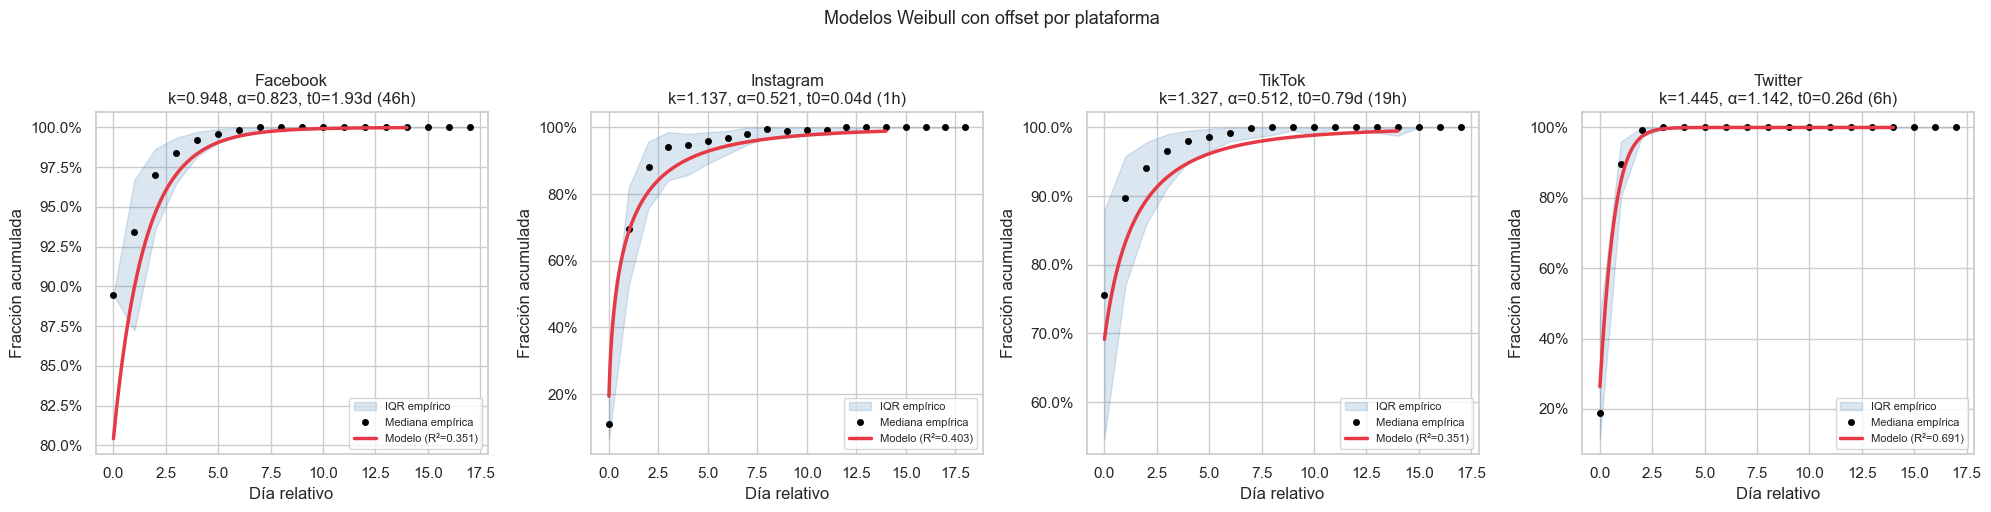
\includegraphics[width=0.90\textwidth]{img/costa_rica_r2_1.png}
  \end{center}
\end{frame}
\makeblue

\setcounter{framenumber}{18}
\makered
\begin{frame}{Etapa 3: Colombia -- infraestructura de extracción}
  \begin{columns}[T]
    \begin{column}{0.52\textwidth}
      \textbf{Tres plataformas monitoreadas}
      \begin{itemize}
        \item \textbf{Facebook} y \textbf{TikTok}: Apify (infraestructura comercial de scraping)
        \item \textbf{Twitter/X}: scraper propio con Playwright (navegador \textit{headless})
        \item \alrt{Instagram excluida}: Meta cerró su API pública para investigadores
              independientes desde 2023
      \end{itemize}
      \vspace{0.3em}
      \textbf{Ventana temporal:} 15 días anteriores al 29 oct.\ 2023
      \vspace{0.3em}
      {\small\textbf{Restauración Weibull:}\\
      Las interacciones brutas se convierten en estimaciones al \textbf{día de la elección},
      descontando el tráfico póstumo acumulado desde oct.\ 2023 hasta la extracción.}
    \end{column}
    \begin{column}{0.44\textwidth}
      \begin{block}{Dataset final}
        \begin{itemize}\small
          \item \textbf{5.776} publicaciones únicas
          \item \hspace{1em} Facebook: \textbf{2.511}
          \item \hspace{1em} Twitter/X: \textbf{2.346}
          \item \hspace{1em} TikTok: \textbf{919}
          \item[\phantom{x}]
          \item 31 ciudades, \textbf{120 candidatos}\\
                (más de 10k votos)
          \item 92,6\% con publicaciones activas
        \end{itemize}
      \end{block}
    \end{column}
  \end{columns}
\end{frame}
\makeblue

\setcounter{framenumber}{20}
\makered
\begin{frame}{Etapa 3: Correlación dominancia digital vs. cuota de voto}
  \begin{center}
    
\includegraphics[height=0.82\textheight]{img/col_scatter_dominancia_votos.png}
  \end{center}
  {\footnotesize\color{subtleGray}\centering
    $\rho = 0{,}70$, 120 candidatos, 31 ciudades \corr{[Corr.\ 2.2]}}
\end{frame}
\makeblue

\setcounter{framenumber}{25}
\makered
\begin{frame}{Dos modelos: reconciliación de coeficientes \corr{[Corr.\ 1.14, 1.15]}}
  \vspace{-0.2em}
  \begin{center}
  \scriptsize
  \rowcolors{2}{tableBand}{white}
  \begin{tabular}{L{4.0cm} C{1.6cm} C{1.4cm} C{1.4cm} C{1.8cm} C{2.2cm}}
    \toprule
    \rowcolor{barBlue}
    {\color{white}\textbf{Especificación}} &
    {\color{white}$\beta_0$} &
    {\color{white}$\beta_1$} &
    {\color{white}$\beta_2$} &
    {\color{white}\textbf{MAE LOCO}} &
    {\color{white}\textbf{Transferible 2026}} \\
    \midrule
    Regresión fraccional simple (Fig.\ 6.4) &
      {N/A} & 0,423 & {N/A} & 11,52 pp & Sí \\
    \rowcolor{tableBand}
    \textbf{ElasticNet 2 vars.\ (modelo final)} &
      0,258 & \textbf{0,111} & \textbf{0,026} & \textbf{9,56 pp} & \textbf{Sí} \\
    ElasticNet 9 vars.\ (pool completo) &
      0,258 & 0,111 & 0,557$^*$ & 9,57 pp & \alrt{No} \\
    \bottomrule
  \end{tabular}
  \end{center}

  {\footnotesize $^*$ $\beta_2 = 0{,}557$: coeficiente del moderador cuando ElasticNet opera
  sobre el pool completo de 9 variables, con variables territoriales como efectos directos.}

  \vspace{0.2em}
  \begin{columns}[T]
    \begin{column}{0.55\textwidth}
      \textbf{¿Por qué el modelo de 9 vars.\ no es transferible a 2026?}
      \begin{itemize}
        \item Retiene «número de candidatos» como efecto directo
        \item En una 2.ª vuelta: exactamente 2 candidatos; constante sin poder discriminador
        \item El modelo de 2 vars.\ retiene solo señal digital pura más moderador de población
      \end{itemize}
    \end{column}
    \begin{column}{0.41\textwidth}
      \begin{alertblock}{Aclaración proactiva}
        Los tres juegos de coeficientes corresponden a \textbf{tres especificaciones distintas},
        no a inconsistencias. La tesis incluye una tabla unificada de reconciliación.
      \end{alertblock}
    \end{column}
  \end{columns}
\end{frame}
\makeblue

\setcounter{framenumber}{26}
\makered
\begin{frame}{Modelado: estabilidad de los coeficientes entre pliegues LOCO-CV}
  \begin{center}
    
\includegraphics[width=0.72\textwidth]{img/col_coef_bootstrap.png}
  \end{center}
  {\footnotesize\color{subtleGray}\centering
    Media $\pm$ IC 95\% del coeficiente en escala logit a través de los 31 pliegues LOCO-CV.
    La dominancia de \textit{likes} ($\beta_1 \approx 0{,}78$) y el moderador ($\beta_2 \approx 0{,}54$)
    son estables. Ningún pliegue invierte el signo de ningún coeficiente.}
\end{frame}
\makeblue

\setcounter{framenumber}{27}
\makered
\begin{frame}{Modelado: diagnóstico del modelo ElasticNet -- LOCO-CV}
  \begin{center}
    
\includegraphics[width=0.90\textwidth]{img/col_loco_residuals.png}
  \end{center}
  {\footnotesize\color{subtleGray}\centering
    Izquierda: predicción vs.\ cuota real (MAE = 9,56 pp).
    Derecha: distribución de residuos centrada en cero (sesgo medio = 0,00 pp).
    El modelo no sobreestima ni subestima sistemáticamente.}
\end{frame}
\makeblue

\setcounter{framenumber}{34}
\makered
\begin{frame}{Próximos pasos y agenda futura}
  \begin{columns}[T]
    \begin{column}{0.48\textwidth}
      \textbf{Validación definitiva, 2027}
      \begin{itemize}
        \item Elecciones territoriales de Colombia 2027
        \item Mismo contexto multi-candidato subnacional
        \item Modelo ya entrenado; evaluación \textbf{ex-ante} estricta
        \item Permitirá aislar el desempeño sin sesgos del filtro retrospectivo
      \end{itemize}
      \vspace{0.4em}
      \textbf{Extensión: nowcasting continuo}
      \begin{itemize}
        \item Ejecutar ELA-NOM cada 24 horas durante la campaña
        \item Arquitectura técnica ya resuelta con el restaurador Weibull
        \item Solo requiere datos de extracción diaria
      \end{itemize}
    \end{column}
    \begin{column}{0.48\textwidth}
      \textbf{Líneas de investigación futura}
      \begin{itemize}
        \item Validación del modelo Weibull en elecciones con distintos perfiles demográficos
        \item Diseño de umbral de inclusión basado en información pre-elección
        \item Inclusión de Instagram cuando Meta reabra el acceso para investigadores
        \item Logit condicional de McFadden como clasificador complementario \corr{[Corr.\ 1.20]}
        \item Análisis de sensibilidad completo sobre la imputación $\varepsilon$ \corr{[Corr.\ 1.13]}
      \end{itemize}
    \end{column}
  \end{columns}
\end{frame}
\makeblue

\setcounter{framenumber}{35}
\makered
\begin{frame}{Cumplimiento de objetivos}
  \vspace{-0.1em}
  \begin{block}{Objetivo general -- \ok{Cumplido}}
    \small Diseñar, implementar y validar un modelo de \textit{nowcasting} electoral
    elección-agnóstico e independiente de encuestas para el entorno colombiano.
  \end{block}
  \vspace{0.2em}
  {\small\textbf{Objetivos específicos:}}
  \vspace{0.1em}
  \begin{center}
  {\setlength{\tabcolsep}{4pt}
  \scriptsize
  \rowcolors{2}{tableBand}{white}
  \begin{tabular}{L{6.2cm} C{1.6cm} L{4.0cm}}
    \toprule
    \rowcolor{barBlue}
    {\color{white}\textbf{Objetivo específico}} &
    {\color{white}\textbf{Estado}} &
    {\color{white}\textbf{Evidencia}} \\
    \midrule
    OE1. Replicar SOMEN-DC y documentar sus limitaciones &
      \ok{Cumplido} & Bolivia 2025 -- PM1, PM2 \\
    OE2. Diseñar restaurador temporal para datos históricos &
      \ok{Cumplido} & Weibull por plataforma -- PM3, P2 \\
    OE3. Construir dataset y validar señal digital en Colombia &
      \ok{Cumplido} & 31 ciudades, $\rho=0{,}70$, $p=0{,}048$ -- P1 \\
    OE4. Seleccionar el modelo de mejor desempeño predictivo &
      \ok{Cumplido} & ElasticNet 2v., MAE=9,56 pp, $R^2=0{,}518$ -- P3 \\
    OE5. Validar transferibilidad a elección no vista &
      \ok{Cumplido} & 2.ª vuelta 2026, MAE=10,98 pp -- PM4 \\
    \bottomrule
  \end{tabular}}
  \end{center}
\end{frame}
\makeblue

% Fix the final counter so totalframenumber evaluates to 37
\setcounter{framenumber}{37}
